\documentclass[10pt,a4paper]{article}
\usepackage[utf8]{inputenc}
\usepackage[french]{babel}
\usepackage[T1]{fontenc}
\usepackage{graphicx}
\usepackage{amsthm}
\usepackage{amssymb}
\usepackage{amsmath}
\usepackage[left=2cm,right=2cm,top=2cm,bottom=2cm]{geometry}
\author{Raphaël Wormer}
\title{Hexaflexagones}
\graphicspath{{Images/}}
\linespread{1.15}
\usepackage{mathtools}



\def\intv#1[#2..#3]{\mathopen{#1[}#2\mathrel{{.}\,{.}}\nobreak#3\mathclose{#1]}}

\begin{document}





\maketitle
\tableofcontents

\paragraph{Remerciements sincères}Céline sans qui ce travail n'aurais pas vu le jour.


\section{Introduction}\label{intro}
	\subsection{Motivations}\label{motiv}
	\subsection{Objectifs}\label{objtf}



\section{Hexaflexagones}\label{hexa-1}


	\subsection{Présentation}\label{hexa-pres}
	
		\subsubsection{Construction et manipulation}\label{constr-1}
			\paragraph{Le trihexaflexagone}

		\subsubsection{Le flexagone à travers les âges}\label{hexa-histo}


	\subsection{Représentations}\label{hexa-repr}
		\paragraph{}Pour comprendre le fonctionnement des flexagones, la première question qui se pose est celle de leur représentation mathématique. Je donne ici les représentations les plus classiques qui serviront dans les applications.
		
		\subsubsection{Patrons}
			\paragraph{}On a vu \ref{constr-1} comment construire les flexagones. Une première remarque est qu'en coupant une charnière entre deux triangles, chaque flexagone se déplie en une bande de triangles colorés.
			
		\subsubsection{Traversée de Tuckerman}
		
		\subsubsection{Diagramme de Tuckey}
		
		\subsubsection{Listes d'Oakley-Wisner}


	\section{Méthodes de construction}
		\subsubsection{Méthode de base}
			\paragraph{}On a déjà décrit cette méthode en \ref{constr-1}
			
		\subsubsection{Reflecto-clonage}
			\paragraph{}Le reflecto clonage est décrit par David King sur sa page, et fût utilisé avec succès par Antonio machin dans son programme hexafind. Il s'agit d'une amélioration de la méthode de base.
			
		\subsubsection{Utilisation des diagrammes}
		
		
	\section{Décoration}
	
	
	
\section{Triangulations de polygones}


	\subsection{Généralités}
		\paragraph{}On ne considère ici que les triangulations de polygones convexes.
		
		
	\subsection{Dénombrement}
	
		\subsubsection{Comptage totale, nombres de Catalan}
			Il est connu que le nombre de triangulations d'un $n$-gone convexe est le nombre de Catalan 
			$\frac{1}{n-1}\binom{2(n-2)}{n-2}$. Je rappelle rapidement une preuve pour comprendre d'où vient ce résultat. On utilisera des arguments combinatoires du même style plus tard.

			Pour $n\in\mathbb{N}$, on note $C_{n}$ le nombre de triangulations d'un $n+2$-gone convexe, avec $C_{0} = 1$ par convention.\\			
			Soit $n \in \mathbb{N}$, $n \geqslant3$, considérons une triangulation  d'un $n$-gone convexe:\\

			Étant donné un côté $[P_{0}P_{1}]$ du polygone, et le sommet $P_{r}$ tel que $\Delta = P_{0}P_{1}P_{r}$ soit un triangle de la triangulation, où $r$ est le nombre de sommets entre $P_{0}$ et $P_{r}$ dans le sens direct.\\
			$\Delta$ sépare la triangulation en deux triangulations de $r+2$ et $n-r-1$ côtés.\\
			\begin{figure}[h]
				\centering
				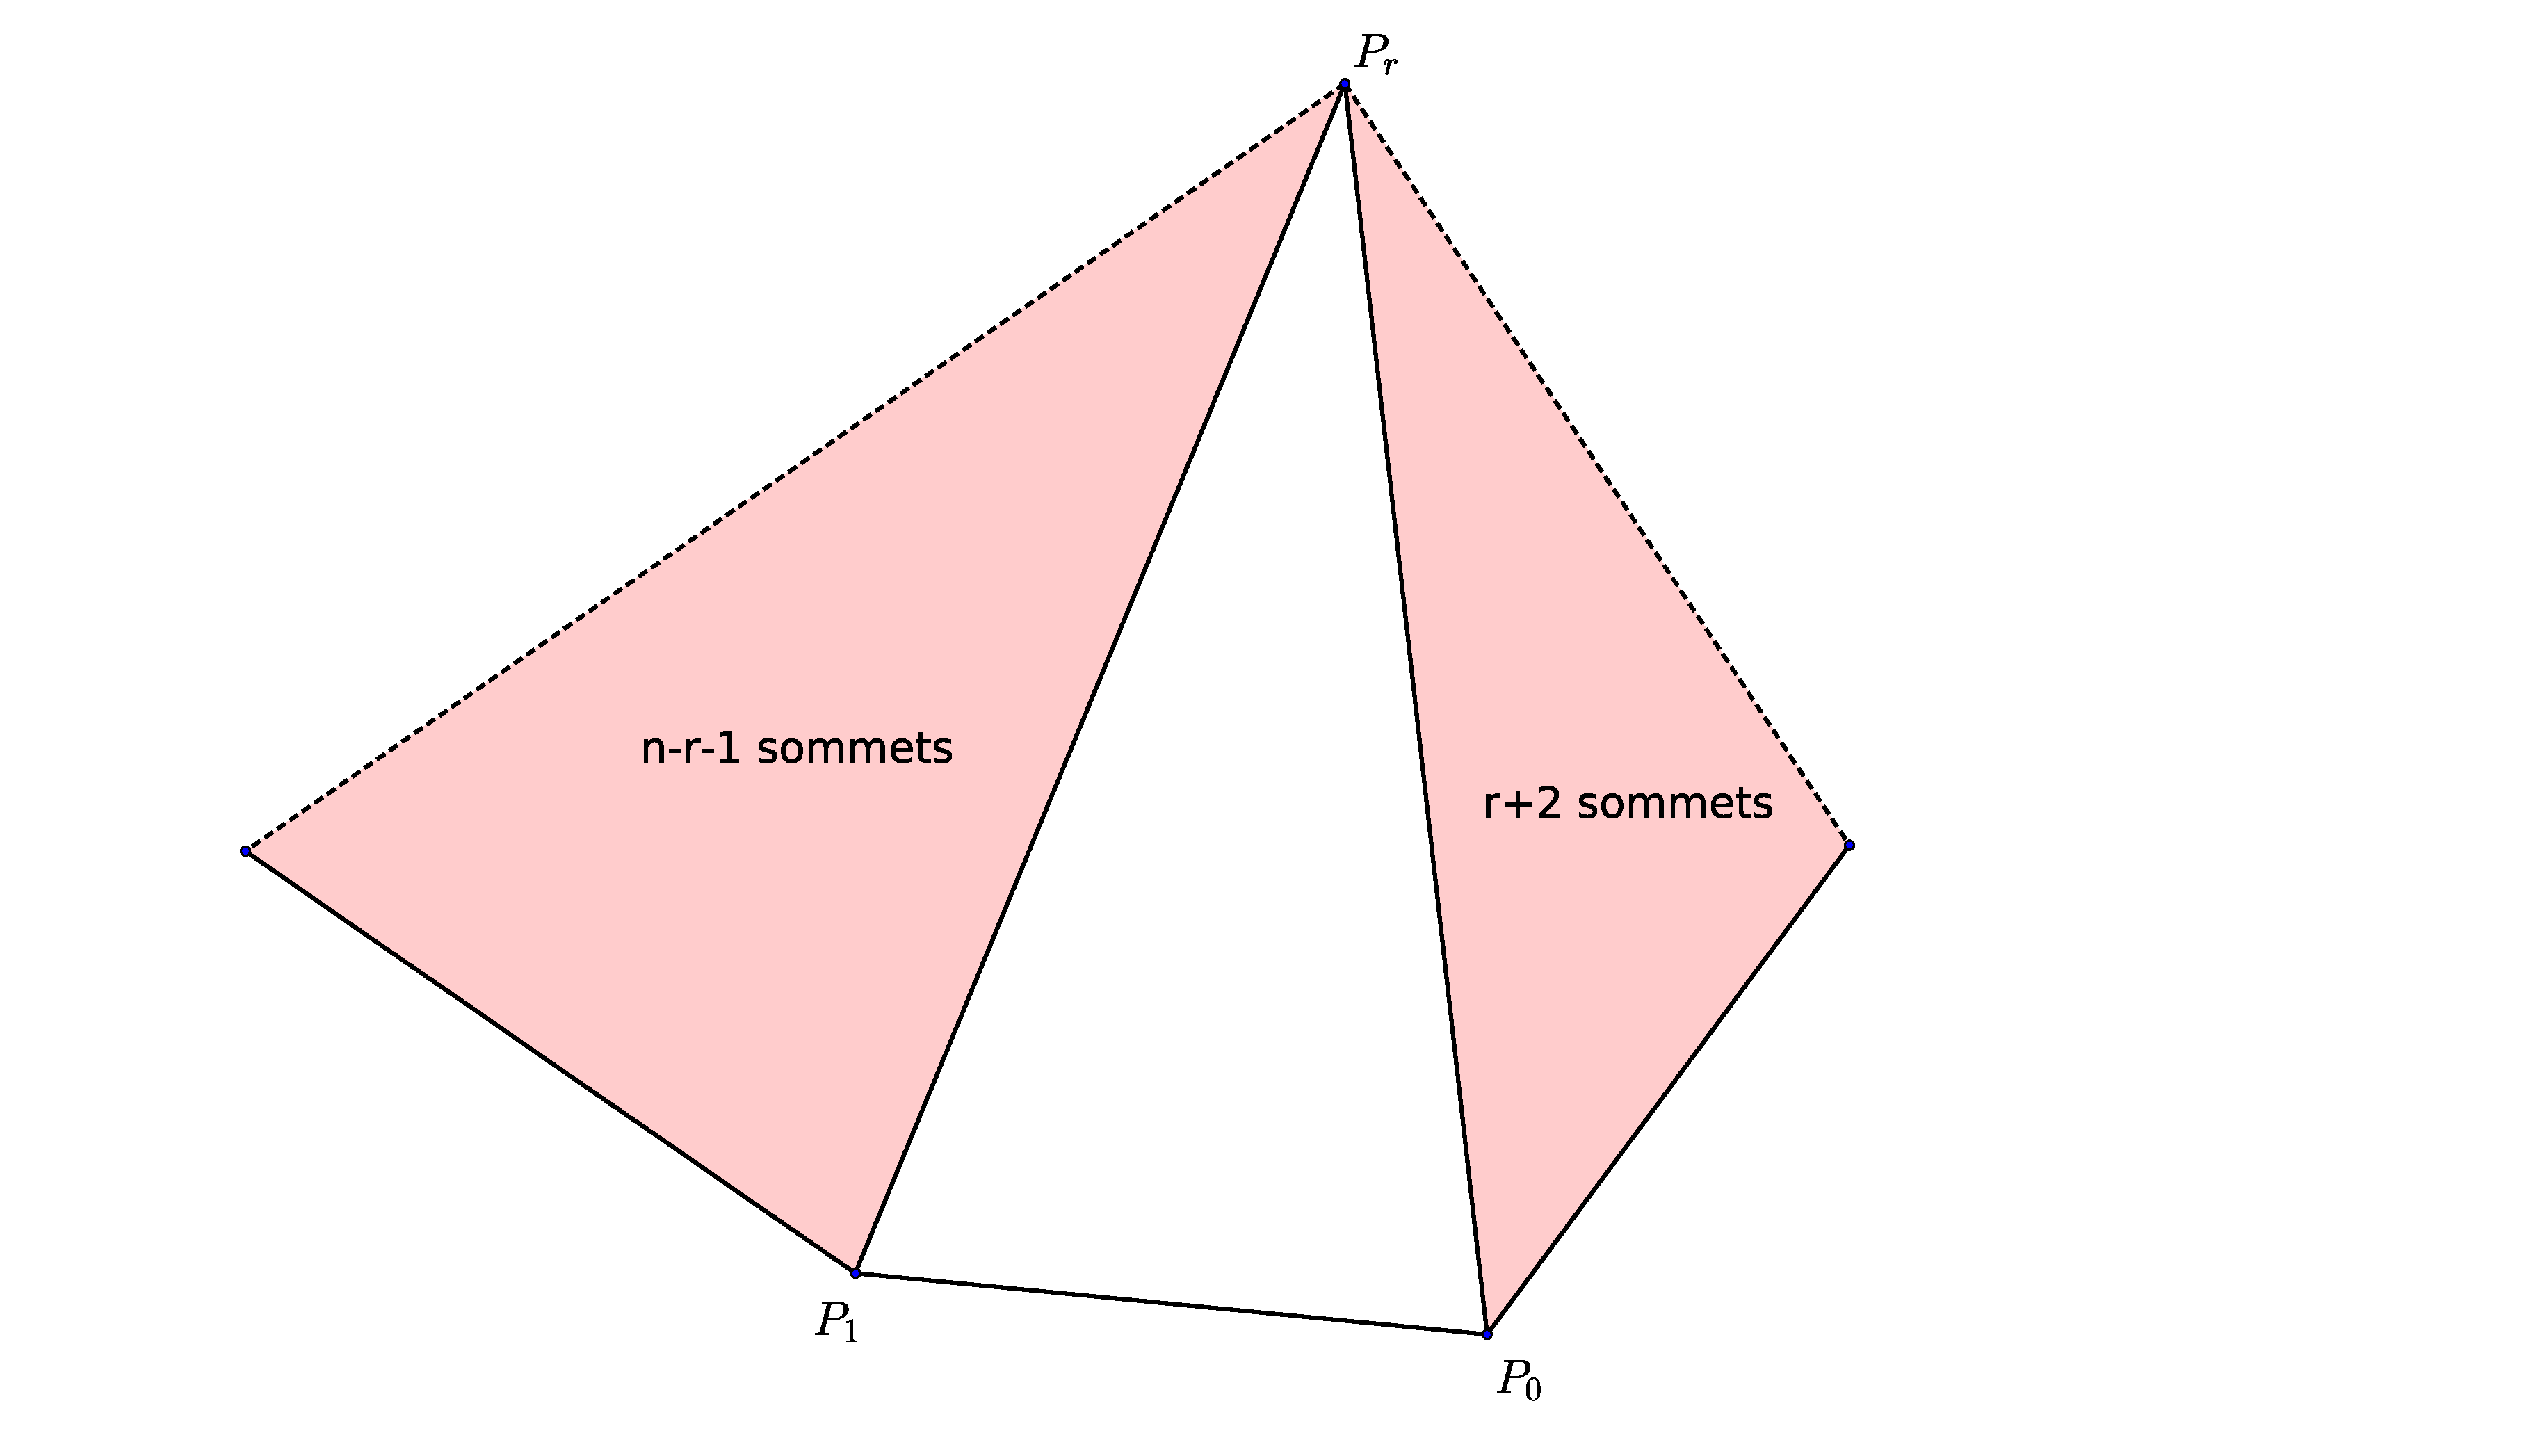
\includegraphics[scale=0.25]{nombres_catalan.eps}
			\end{figure}
			Pour $r\in [0,\ldots,\:n-3]$, il y bijection entre les triangulations d'un $n$-gone convexe et les couples $(T_{n-r-1},T_{r+2})$ où $T_{i}$ est une triangulation d'un $i$-gone convexe.\\
			Il y a donc $C_{r}C_{n-r-3}$ triangulations du $n$-gone, $r$ étant fixé.\\
			Chaque choix de $r$ défini des ensembles de triangulations disjoints, d'où la formule de récurrence
			\[C_{n-2} = \sum_{r=0}^{n-3}{C_{r}C_{n-3-r}}\] 
			\[soit\;
				\begin{dcases*}
		        C_{0} = 1\\
		        \forall n\in\mathbb{N},\; C_{n+1} = \sum_{r=0}^{n}{C_{r}C_{n-r}}
		        \end{dcases*}
			\]
			Notons alors la série formelle $$F(X) = \sum_{n=0}^{+\infty}{C_{n}X^{n}}$$
			

		\subsubsection{Action de groupe, Classes de symétrie}



\section{Programmation}

	\subsection{Structures de données}
	
	\subsection{•}





\end{document}